\chapter{Struktur}\label{Ch:Struktur}\index{Struktur}
\lettrine{Z}{entrales} Element sind die \DEF{SL-Erzählphasen}\index{SL-Erzählphase}. Mit Hilfe von Erzählphasen bringt der SL die Story voran. Hierdurch legt der SL die Szenen fest, d.\,h. er bestimmt Ort, Zeit, Charaktere usw. der nächsten Szene. Dabei sind Orts- und Zeitwechsel (z.\,B. R"uckblenden oder Zeitspr"unge) möglich. Beginn und Ende eines jeden Abenteuers ist eine solche Erzählphase. Außerdem leiten sie jeweils zum nächsten Konflikt oder zum nächsten freien Spiel über (s.\,u.). Dabei sind die Erzählphasen zwar zentrale Elemente des Spiels, sollen aber im Gegensatz zu den Konflikten und zum freien Spiel nicht den Hauptteil des Spiels ausmachen. In den Erzählphasen beschreibt der SL, was die Charaktere wahrnehmen und wie sie sich verhalten.

Auch Szenen, die an einem anderen Ort spielen, sind als Erz"ahlung m"oglich. Dadurch k"onnen Informationen, die die Charaktere nicht haben, an die \emph{Spieler} weitergegeben werden. Solche Erz"ahlphasen k"onnen beispielsweise genutzt werden, um den Spielern die Dringlichkeit eines bestimmten Vorgehens nahezubringen. Nat"urlich sollte der Spielleiter darauf achten, dass mit solchen Szenen die Spannung gesteigert und nicht durch zu viel Information gesekt wird.

Dagegen sollen \DEF{Konflikte}\index{Konflikt} das Herz eines Rollenspiels sein. Wie enden kritische Situationen? Ich möchte grundsätzlich zwei Konfliktarten unterscheiden: Nebenkonflikt und Hauptkonflikt.

Dabei dienen \DEF{Nebenkonflikte}\index{Nebenkonflikt} dazu, relativ unwichtige Konflikte zu modellieren. Es sind die Konflikte, die den Helden behindern und den Weg zum eigentlichen Konflikt spannend machen. Eigentlich ist klar, wie ein solcher Nebenkonflikt ausgeht: Die Helden gewinnen. Dabei können sie sich aber in weitere Konflikte verstricken, Wunden davontragen oder auch mal besonders erfolgreich sein. Es ist die Räuerbande auf dem Weg zum Dachenhort, es ist der einstürzende Tempel, dem die Helden entfliehen müssen oder die Torwache, die bestochen werden muss.

Nebenkonflikte in der Literatur werden manchmal länger, manchmal kürzer beschrieben. Auch das ist mit den Konfliktregeln möglich. Die Länge eines Nebenkonfliktes entscheidet darüber, wie viele Nebenwirkungen ein solcher Konflikt haben kann. Also: Lange Nebenkonflikte sind wichtiger als kurze. Eine besonders kurze Form von Konflikten stellen die \DEF{Kurzkonflikte}\index{Kurzkonflikt} dar, die in gewisser Weise nur noch das Ende eines Nebenkonfliktes darstellen.

\DEF{Hauptkonflikte}\index{Hauptkonflikt} dagegen sind echte Scheidewege. Ihr Ausgang ist unklar, hier wird es richtig spannend. Kann der Held den Dämonenmeister bezwingen oder schafft dieser eventuell die Flucht? Wie schneidet der Held beim Bardenwettstreit ab? Reicht die Argumentation aus, um den Mörder seiner gerechten Strafe zuzuführen?

\begin{figure}[t!]
\centerline{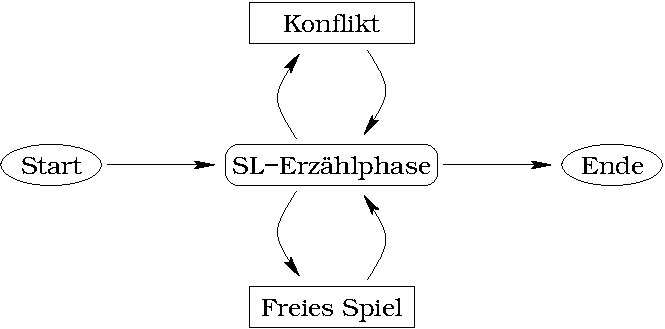
\includegraphics[width=0.8\textwidth]{pics/flowchart}}
\caption{Jedes Abenteuer beginnt und endet mit einer SL-Erzählphase. Dazwischen liegen immer wieder Konflikte und freies Spiel, wobei die Erzählphasen die Übergänge dazwischen darstellen.}

\medskip
\hrule
\end{figure}

Darüberhinaus gibt es noch \DEF{freies Spiel}\index{freies Spiel}, welches außerhalb von Konflikten steht. Dabei spielen die Spieler einfach in der gegebenen Szene die Charaktere frei aus. Hier können Entscheidungen über das weitere Vorgehen o.ä. entschieden werden.

Um eine klare Strukturierung des Spieles hinzubekommen, gibt es \DEF{Schlüsselworte}\index{Schlüsselworte} und Gesten. Damit leitet der SL von einer Phase zur nächsten über. Dazu sollte er sich -- falls er nicht die volle Aufmerksamkeit aller Spieler hat -- durch kurzes Räuspern oder Aufsetzen die Aufmerksamkeit sichern. Dann spricht er mit klarer Stimme und einer zur Stimmung passenden Stimme den Schlüsselsatz. So weiß jeder, in welcher Phase des Spiels man sich gerade befindet.

\subsection{Die Schlüsselworte in der Übersicht}
\begin{description}
\item[Freies Spiel:] ``Was wollt ihr tun?''

\item[Einleitung eines Konfliktes:] ``Es kommt zu Schwierigkeiten. Dein/Euer Ziel ist es, \dots''

\item[SL-Erzählphase:] ``Nachdem du/ihr \dots''. Zur Verdeutlichung, dass in eine SL-Erz"ahlphase "ubergeleitet wird, kann der SL zus"atzlich die Hand heben.
\end{description}


\subsection{Beispiele}
\begin{beispiel}
\paragraph{Beispiel 1:} Der SL m"ochte den Spielern Gelegenheit geben, das weitere Vorgehen zu planen. Dazu beschreibt er, wie sich die Helden eine Taverne betreten. \emph{``\dots Rauchgeschw"angerte Luft schl"agt euch entgegen. Die fast heruntergebrannten Kerzen an den W"anden k"onnen den Raum nur schwer erhellen und tauchen ihn in ein unwirkliches Licht. An den niedrigen Tischen sitzen kaum erkennbare, dunkle Gestalten. `In was sind wir jetzt hineingeraten', denkt ihr euch. Da dr"ohnt aus dem hinteren Teil des Raumes die Stimme des Wirts: `Heda, Fremde! Setzt euch doch. Ich habe hier hinten noch einen guten Tisch f"ur Euch!' Ihr nehmt dankend an und setzt euch. {\bfseries Was wollt ihr tun?}''}

\paragraph{Beispiel 2:} Die Spieler entscheiden sich im Laufe ihrer Planung, Haken-Hoss aufzusuchen und ihm geh"orig eins zu verpassen. Dazu hatten sie bereits ein Boot am Ufer versteckt, mit dem sie zur Insel "ubersetzen wollen. Der SL muss also zun"achst eine SL-Erz"ahlphase einleiten, die er nutzen will, "uberraschenderweise eine Kneipenschl"agerei einzuleiten, denn einer der G"aste hat die Helden belauscht und will sie von ihrem Vorhaben abbringen: \emph{``{\bfseries Nachdem ihr} beschlossen habt, Haken-Hoss aufzusuchen und eure Humpen geleert habt, steht ihr auf, als pl"otzlich ein Raunen durch den Raum geht. Das Kratzen von St"uhlen und Tischen, die zur Seite geschoben werden, erf"ullt die Taverne. \textbf{Es kommt zu Schwierigkeiten. Euer Ziel ist es,} heil aus der Kneipenschlägerei herauszukommen.''}

\paragraph{Beispiel 3:} Nach dem Kampf erz"ahlt der SL, wie die Helden auf dem Weg zu Haken-Hoss das bereit gelegte Boot benutzen um damit zur Insel "uberzusetzen. \emph{``\dots steigt ihr alle ins Boot und legt ab. Das Meer ist heute unruhig, das Boot l"asst sich nicht so einfach steuern, wie ihr gedacht habt. {\bfseries Es kommt zu Schwierigkeiten. Euer Ziel ist es,} ohne zu kentern am Ufer der Insel anzukommen. ''}
\end{beispiel}

\begin{design}
\subsubsection{Designanmerkung: Phasen und Schl"usselworte}

Der Vorteil einer klaren Trennung der verschiedenen Phasen liegt auf der Hand: Der Spielleiter beh"alt die Herrschaft "uber den Plot und kann genau vorgeben, in welchem Rahmen die Spieler ihre Charaktere ausspielen d"urfen.

Die Schl"usselworte wiederum dienen dazu, das Spiel so unauff"allig wie m"oglich zu strukturieren, um den Spielfluss m"oglichst wenig zu st"oren. Dadurch ist allen Beteiligten auch ohne Out-Time Anmerkungen immer klar, in was f"ur einer Art von Spiel sie sich gerade befinden: Macht der SL nur eine Anmerkung zum freien Spiel oder leitet er eine SL-Erz"ahlphase ein? Kommt jetzt ein Konflikt oder kann ich meinen Charakter frei ausspielen?
\end{design}

\begin{optional}
\section{Optional: Andere Schl"usselworte}

Es ist im Allgemeinen problemlos m"oglich, auch andere Schl"usselworte zu benutzen. Wahrscheinlich wird sich auch mit der Zeit ein eigener Stil einschleifen, so dass jeder Spieler immer genau wei"s, in welcher Phase sich das Spiel gerade befindet.
\end{optional}


